\documentclass[a4paper,12pt]{report}
% safe参数解决与\!在内的多个冲突
% \sups命令可能被重定义,xeCJK放在tipa后
\usepackage[safe]{tipa}

% 中文支持
\usepackage[slantfont,boldfont]{xeCJK}
	\setCJKmainfont[BoldFont=SimHei,ItalicFont=KaiTi]{SimSun}
	\setCJKmathfont{STXinwei}
\usepackage{indentfirst}

% 数学环境
\usepackage{amsmath}
  \newcommand{\ue}{\mathrm{e}}
  \newcommand{\ud}{\mathop{}\negthinspace\mathrm{d}}
\usepackage{amssymb}
\usepackage{mathrsfs} % 线性代数字体
    % overline的替代命令
\newcommand{\closure}[2][3]{{}\mkern#1mu\overline{\mkern-#1mu#2}}
\usepackage{yhmath} % 左下-右上省略号
\usepackage{mathtools} % dcases环境
\usepackage{amsthm} % 定理环境
  \theoremstyle{definition}\newtheorem{laws}{Law}[section]
  \theoremstyle{plain}\newtheorem{ju}[laws]{Jury}
  \theoremstyle{remark}\newtheorem*{marg}{Margaret}
\usepackage{esint} % 多重积分,需放在amsmath后

% 下划线宏包
\usepackage{ulem}
% LaTeX符号宏包
\usepackage{hologo}
	\newcommand{\xelatex}{\Hologo{XeLaTeX}}
	\newcommand{\bibtex}{\Hologo{BibTeX}}
% 其他符号
\usepackage{wasysym}
% 带箱小页
\usepackage{boxedminipage}
% 绘图
\usepackage{tikz}
	\usetikzlibrary{calc}
	\newcommand{\tikzline}[1]{{#1\tikz{\draw[#1,line width=9](0,0)--(0.5,0);}}, }

% 奇怪的小定义
\newcommand{\dpar}{\\ \mbox{}}	% 空两行
\newcommand{\qd}[1]{{\bfseries{#1}}}	% 强调
\newcommand{\co}[1]{{\bfseries{#1}}}   % Style of concept
\newcommand{\RED}[1]{{\color{red}{#1}}}
\newcommand{\cmmd}[1]{\fbox{\texttt{\char92{}#1}}}
\newcommand{\charef}[1]{第\ref{#1}章}
\newcommand{\secref}[1]{第\ref{#1}节}
\newcommand{\pref}[1]{第\pageref{#1}页}
\newcommand{\fref}[1]{图\ref{#1}}
\newcommand{\tref}[1]{表\ref{#1}}

% 编号列表宏包,并自定义了三个列表
%\usepackage[inline]{enumitem}
%	\setlist[enumerate]{label=\arabic* - ,font=\bfseries,itemsep=0pt}
%	\setlist[itemize]{label=$\bullet$,font=\bfseries,leftmargin=\parindent}
%	\setlist[description]{font=\bfseries\uline}
%
%\newenvironment{fead}{\setlength{\parskip}{0pt}
%	\begin{description}[font=\bfseries\uline,labelindent=\parindent]
%		\setlength{\itemsep}{0pt}\setlength{\parsep}{0pt}\setlength{\parskip}{0pt}}
%	{\end{description}}
% 带宽度的
\newenvironment{para}{\setlength{\parskip}{0pt}
	\begin{description}[font=\bfseries\ttfamily]
		\setlength{\itemsep}{0pt}\setlength{\parsep}{0pt}\setlength{\parskip}{0pt}}
	{\end{description}}
\newenvironment{feae}{\setlength{\parskip}{0pt}
	\begin{enumerate}[font=\bfseries,labelindent=0pt]}
	{\end{enumerate}}
\newenvironment{feai}{\setlength{\parskip}{0pt}
	\begin{itemize}[font=\bfseries]
		\setlength{\itemsep}{0pt}\setlength{\parsep}{0pt}\setlength{\parskip}{0pt}}
	{\end{itemize}}
\newenvironment{inlinee}
{\begin{enumerate*}[label=(\arabic*), font=\rmfamily, before=\unskip{:},itemjoin={{;}},itemjoin*={{,以及:}}]}
	{\end{enumerate*}。}

% 目录和章节样式
\usepackage{titlesec}
\usepackage{titletoc}   % 用于目录

\titlecontents{chapter}[1.5em]{}
	{\contentslabel{1.5em}}{\hspace*{-2em}}{\hfill\contentspage}
	
\titlecontents{section}[3.3em]{}
	{\contentslabel{1.8em}}
	{\hspace*{-2.3em}}
	{\titlerule*[8pt]{$\cdot$}\contentspage}
%	
\titlecontents{subsection}[2.5em]{\small}
	{\thecontentslabel{} }
	{}
	{\titlerule*[5pt]{$\cdot$}\contentspage}
 %章节样式
\setcounter{secnumdepth}{3} % 一直到subsubsection
\newcommand{\chaformat}[1]{%
	\parbox[b]{.5\textwidth}{\hfill\bfseries #1}%
	\quad\rule[-12pt]{2pt}{70pt}\quad
	{\fontsize{60}{60}\selectfont\thechapter}}
\titleformat{\chapter}[block]{\hfill\LARGE\sffamily}{}{0pt}{\chaformat}[\vspace{2.5pc}\large
	\startcontents\printcontents{}{1}{\setcounter{tocdepth}{2}}]
%\titleclass{\section}{top}
%\titleformat{\section}{\Large\bfseries}{\thesection}{0.5em}{}
\titleformat*{\section}{\centering\Large\bfseries}
\titleformat{\subsubsection}[hang]{\bfseries\large}{\rule{1.5ex}{1.5ex}}{0.5em}{}
% 扩展章节
\newcommand{\starsec}{\noindent\fbox{\S\textit{注意:本章节是一个扩展阅读章节。}}
	\\ \mbox{}}

\renewcommand{\contentsname}{目录}
	\renewcommand{\tablename}{表}
	\renewcommand\arraystretch{1.2}	% 表格行距
	\renewcommand{\figurename}{图}
% 设置不需要浮动体的表格和图像标题
\setlength{\abovecaptionskip}{5pt}
\setlength{\belowcaptionskip}{3pt}
\makeatletter
\newcommand\figcaption{\def\@captype{figure}\caption}
\newcommand\tabcaption{\def\@captype{table}\caption}
\makeatother
% 图表
\usepackage{array,multirow}
  \setlength\extrarowheight{2pt} % 行高增加
\usepackage{longtable}
\usepackage{graphicx}
  \graphicspath{{./tikz/}}
% 页面修正宏包
\usepackage[top=1in]{geometry}

% 代码环境
\usepackage{listings}
% Avoid copy line numbers of the listing code (Invalid for SumatraPDF Reader)
\usepackage{accsupp}
	\newcommand{\emptyaccsupp}[1]{\BeginAccSupp{ActualText={}}#1\EndAccSupp{}}
% Color
\usepackage{xcolor}
	\definecolor{commentcolor}{RGB}{85,139,78}
	\definecolor{numbercolor}{RGB}{166,206,168}
	\definecolor{stringcolor}{RGB}{206,145,108}
	\definecolor{keywordcolor}{RGB}{34,34,250}
	\definecolor{backcolor}{RGB}{220,220,220}
	\definecolor{packagecolor}{RGB}{0,128,0}
	\definecolor{envicolor}{RGB}{185,70,15}
% LaTeX Code Style
%\lstset{language=[LaTeX]TeX,
%		basicstyle=\small\ttfamily,
%		commentstyle=\color{commentcolor},
%		keywordstyle=\color{keywordcolor},
%		stringstyle=\color{stringcolor},
%		showstringspaces=false,
%		% Package/Tikz-Lib Using
%		classoffset=0,
%		morekeywords={begin,end,usetikzlibrary},
%		keywordstyle=\color{keywordcolor},
%		classoffset=1,
%		morekeywords={article,report,book,
%			xeCJK,tikz,
%			calc},
%		keywordstyle=\color{packagecolor},
%		classoffset=2,
%		morekeywords={document,tikzpicture},
%		keywordstyle=\color{envicolor},
%		% Line Number Style
%		numbers=left,
%		numberstyle=\tiny\emptyaccsupp,
%		stepnumber=1,
%		% Frame and Background Color
%		frame=single,
%		framerule=0pt,
%		backgroundcolor=\color{backcolor},
%		% Spaces
%		% belowskip=\medskipamount,
%		emptylines=1,
%		escapeinside=``}

\lstnewenvironment{latex}[1]{\lstset{#1}}{}
\newcommand{\latexline}[1]{{\lstinline[language=TeX,basicstyle=\small\ttfamily]{#1}}}

% Tikz Code
\lstdefinelanguage{tikzlang}{
	classoffset=0, % 蓝色的keyword
	morekeywords={begin,end,newcommand,
		draw,node,coordinate,tikzstyle,foreach},
	keywordstyle=\color{keywordcolor},
	classoffset=1, % 棕色的其他关键字
	morekeywords={tikzpicture,grid,at,
		thick,thin,very,ultra,
		red,green,yellow,blue,cyan,magenta,black,
		    gray,darkgray,lightgray,brown,lime,
		    olive,orange,pink,purple,teal,violet,white},
	keywordstyle=\color{envicolor},
	morecomment=[l]{\%},
	morecomment=[s]{/*}{*/},
	morestring=[b]',
	% Escape
	escapeinside=``
}
\lstnewenvironment{tikzcode}[1]{\lstset{language=tikzlang,basicstyle=\small\ttfamily,
		breaklines=true,%backgroundcolor=\color{white},
		linewidth=0.7\linewidth,#1}}{}

% 附录
\usepackage{appendix}

% 行号
\usepackage{lineno}

% 代码输入环境
%\usepackage{verbatim,xcolor}
%\newbox\savedlines
%\newtoks\savedtokens
%\makeatletter
%\def\codeshow{%
%\global\savedtokens={}%
%\def\verbatim@processline{%
%{\setbox0=\hbox{\the\verbatim@line}%
%\hsize=\wd0
%\the\verbatim@line\par}%
%\global\savedtokens=\expandafter{\the\expandafter\savedtokens\the\verbatim@line^^J}}%
%\@tempswatrue
%\setbox0=\vbox\bgroup\parskip=0pt\topsep=0pt\partopsep=0pt
%\verbatim}
%\def\endcodeshow{\endverbatim%
%\unskip\setbox0=\lastbox\egroup
%\global\setbox\savedlines=\box0
%\addvspace{1em}\par\noindent%
%\colorbox{lightgray}{%
%\begin{minipage}{.55\textwidth}{\usebox\savedlines}\end{minipage}}%
%\hfill\fbox{\parbox{.40\textwidth}%
%{\scantokens\expandafter{\the\savedtokens\unskip\endinput}}}%
%\par\addvspace{1em}}
%\makeatother

% 引用
\usepackage[colorlinks,bookmarksopen=true,bookmarksnumbered=true]{hyperref}

\usepackage{algorithm}
\usepackage{amsmath,bm}
\usepackage{algorithmic}
\usepackage{fancybox}
\usepackage{listings}
\usepackage{xcolor}
\usepackage{diagbox}
\usepackage{amssymb}
\usepackage{amsmath}
\usepackage{amsthm}
\usepackage{empheq}
\usepackage[framemethod=tikz]{mdframed}
\usepackage{mathtools}

\definecolor{ocre}{RGB}{243,102,25}
\definecolor{mygray}{RGB}{243,243,244}

\newcommand*\mymathbox[1]{%
  \fcolorbox{ocre}{mygray}{\hspace{1em}#1\hspace{1em}}}

\newtheoremstyle{mystyle}
  {\topsep}
  {\topsep}
  {\normalfont}
  {}
  {\sffamily\bfseries}
  {.}
  {.5em}
  {{\color{ocre}\thmname{#1}~\thmnumber{#2}}\thmnote{\,--\,#3}}%
\theoremstyle{mystyle}
\newmdtheoremenv[
  backgroundcolor=mygray,
  linecolor=ocre,
  leftmargin=20pt,
  innerleftmargin=0pt,
  innerrightmargin=0pt,
  ]{theo}{Theorem}[section]

\lstset{
columns=flexible,
numbers=left,
numberstyle=\footnotesize\color{darkgray}, 
basicstyle=\small\ttfamily,
stringstyle=\color{purple},
keywordstyle=\color[RGB]{40,40,255}\bfseries,
commentstyle=\it\color[RGB]{0,96,96},  
stringstyle=\rmfamily\slshape\color[RGB]{128,0,0}, 
showstringspaces=false,      
% directivestyle=\color{blue},
frame=shadowbox,
%framerule=0pt,
backgroundcolor=\color[RGB]{245,245,244},
escapeinside=``, %逃逸字符(1左面的键),用于显示中文
breaklines,
extendedchars=false,
%解决代码跨页时,章节标题,页眉等汉字不显示的问题
xleftmargin=2em,xrightmargin=2em,
aboveskip=1em,%设置边距
tabsize=4, %设置tab空格数  
showspaces=false %不显示空格 
rulesepcolor=\color{red!20!green!20!blue!20}
%rulesepcolor=\color{brown}
}


\title{数值分析第三次大作业}
\author{张晋\\学号:15091060}
\date{最后更新于:\today}
\begin{document}

\maketitle

\tableofcontents


\newpage

\chapter{题目}
关于$x,y,t,u,v,w$的下列方程组:

\[\left\{ \begin{array}{l}
0.5\cos t + u + v + w - x = 2.67\\
t + 0.5\sin u + v + w - y = 1.07\\
0.5t + u + \cos v + w - x = 3.74\\
t + 0.5u + v + \sin w - y = 0.79
\end{array} \right.\]

以及关于$z, t, u$的下列二维数表确定了一个二元函数
$z=f(x,y)$。
\begin{table}[htbp]
  \centering
  \caption{二维数表}
    \begin{tabular}{|c|c|c|c|c|c|c|}
    \hline
    \diagbox{t}{z}{y}& 0     & 0.4   & 0.8   & 1.2   & 1.6   & 2 \\
    \hline
    0     & -0.5  & -0.34 & 0.14  & 0.94  & 2.06  & 3.5 \\
    \hline
    0.2   & -0.42 & -0.5  & -0.26 & 0.3   & 1.18  & 2.38 \\
    \hline
    0.4   & -0.18 & -0.5  & -0.5  & -0.18 & 0.46  & 1.42 \\
    \hline
    0.6   & 0.22  & -0.34 & -0.58 & -0.5  & -0.1  & 0.62 \\
    \hline
    0.8   & 0.78  & -0.02 & -0.5  & -0.66 & -0.5  & -0.02 \\
    \hline
    1     & 1.5   & 0.46  & -0.26 & -0.66 & -0.74 & -0.5 \\
    \hline
    \end{tabular}
  \label{tab:addlabel}
\end{table}

\begin{enumerate}
\item 试用数值方法求出$f(x, y)$在区域
$D = \{ (x,y)|0 \le x \le 0.8,0.5 \le y \le 1.5\}$上的一个近似表达式:
\[p(x,y) = \sum_{r = 0}^k\sum_{s = 0}^k {{c_{rs}}{x^r}{y^s}} \]
要求$p(x,y)$最小的$k$值达到以下的精度:
\[\sigma  = \sum\limits_{i = 0}^{10} {\sum\limits_{j = 0}^{20} {[f({x_i},{y_j}) - p} } ({x_i},{y_j}){]^2} \le {10^{ - 7}}\]
其中,${x_i} = 0.08i,{y_j} = 0.5 + 0.05j$

\item 计算$f(x_i^{\ast},y_j^{\ast}),p(x_i^{\ast},y_j^{\ast})\qquad (i = 1, 2,\cdots,8;j = 1,2,\cdots,5)$的值,以观察$p(x,y)$逼近$f(x,y)$的效果,其中,$x_i^{\ast}=0.1i,y_j^{\ast}=0.5+0.2j$
\end{enumerate}


\subsection*{说明:}
\begin{enumerate}
\item 用迭代方法求解非线性方程组时,要求近似解向量
${\bm{x}^{(k)}}$满足以下精度
\[\dfrac{\|{\bm{x}^{(k)}} - {\bm{x}^{(k - 1)}}\|_{\infty }}{\|{\bm{x}^{(k)}}\|_{\infty }} \le {10^{ - 12}}\]

\item 作二元插值时,要使用分片二次代数插值。

\item 要由程序自动确定最小的$k$值。

\item 打印以下内容:

\begin{enumerate}
\item 全部源程序;

\item 数表:$\{{x_i},{y_j},f({x_i},{y_j})\}\qquad (i = 0,1,2,\cdots,10;j = 0,1,2,\cdots,20)$;

\item 选择过程的$k,\sigma$值;

\item 达到精度要求时的$k$和$\sigma$值以及$p(x,y)$中的系数
$c_{rs}(r = 0,1,\cdots,k;s = 0,1,\cdots,k)$;

\item 数表:$\{x_i^{\ast},y_j^{\ast},f(x_i^{\ast},y_j^{\ast}),p(x_i^{\ast},y_j^{\ast})\}\qquad (i = 1, 2,\cdots,8;j = 1,2,\cdots,5)$。

\end{enumerate}
\item 采用$f$型输出$x_i,y_j,x_i^{\ast},y_j^{\ast}$的准确值,其余实型数采用$e$型输出并且至少显示12位有效数字。
\end{enumerate}


\newpage
\chapter{算法设计方案}
\section{方案综述}
\begin{enumerate}
\item 将${x_i} = 0.08i,{y_j} = 0.5 + 0.05j\quad (i=0,1,\cdots,10;j=0,1,\cdots,20)$代入非线性方程组(\ref{e1})中,用\hyperref[sec:Newton]{Newton迭代法}解出$t_{ij}$和$u_{ij}$;

\item 对数表$z(t,u)$进行\hyperref[sec:Interpolation]{分片双二次插值},求得$z_{ij}=\hat{z}(t_{ij},u_{ij})$

\item 根据$z_{ij}$的值进行\hyperref[sec:qmnh]{曲面拟合},要求精度
$\sigma \le 10^{-7}$
,得拟合函数
\[p(x,y) = \sum_{r = 0}^k\sum_{s = 0}^k {{c_{rs}}{x^r}{y^s}} \]

\item 
创建新的数据点集$x_i^{\ast}=0.1i,y_j^{\ast}=0.5+0.2j\quad (i = 1, 2,\cdots,8;j = 1,2,\cdots,5)$,
并代入非线性方程组(\ref{e1})中,用\hyperref[sec:Newton]{Newton迭代法}解出$t^{\ast}$和$u^{\ast}$,
再用\hyperref[sec:Interpolation]{分片双二次插值}计算出$f(x^{\ast},y^{\ast})$,将其与$p(x^{\ast},y^{\ast})$输出并观察比较。\footnote{算法流程图见第\pageref{flow}页。}
\end{enumerate}




\newpage
\begin{figure}[h]
\small
\centering
\label{flow}
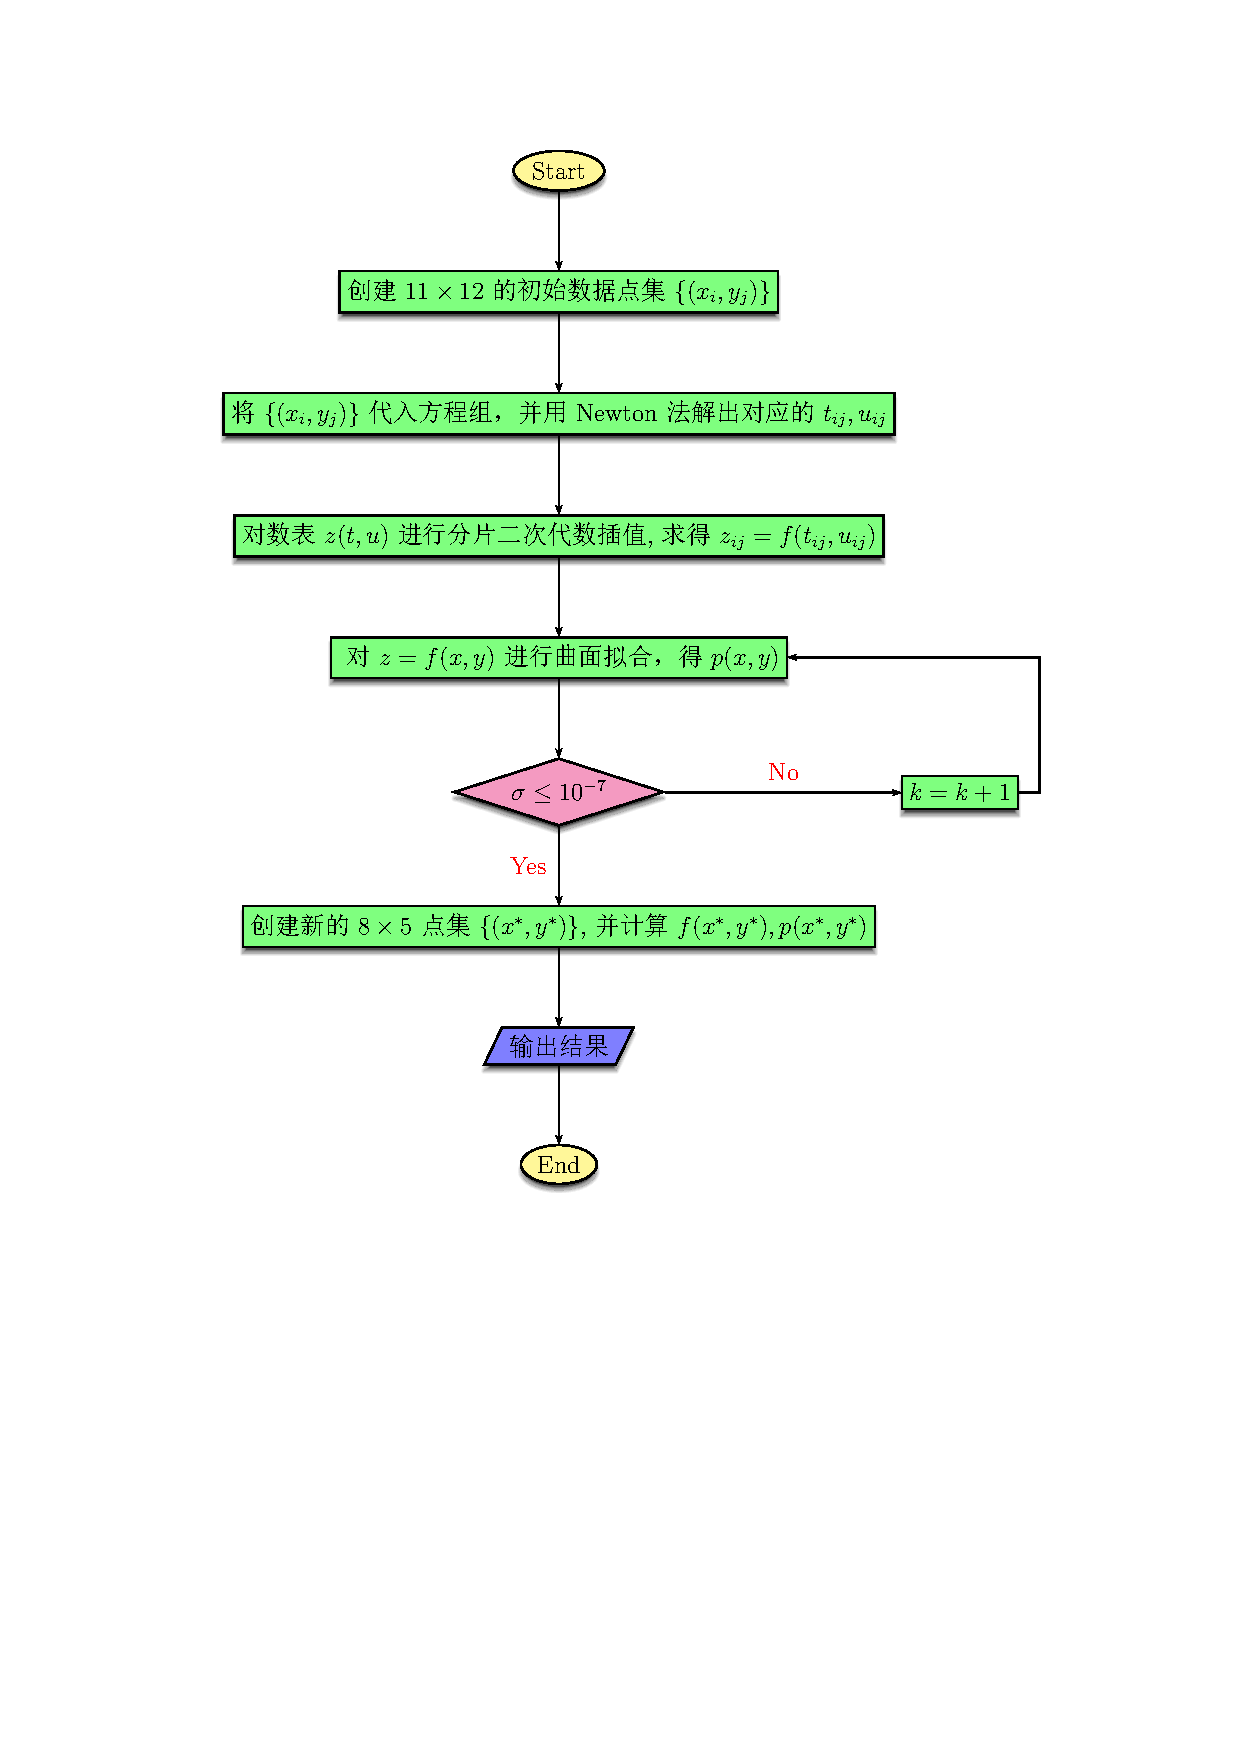
\includegraphics[width=17cm]{flow1}
\end{figure}

\newpage
\section{Newton迭代法}
\label{sec:Newton}
\begin{equation}
\label{e1}
\left\{ \begin{array}{l}
0.5\cos t + u + v + w - x = 2.67\\
t + 0.5\sin u + v + w - y = 1.07\\
0.5t + u + \cos v + w - x = 3.74\\
t + 0.5u + v + \sin w - y = 0.79
\end{array} \right.
\end{equation}


对于该非线性方程组方程组来说,$x,y$为已知量,
需解出$t,u,v,w$。

设$\bm{x}= {(t,u,v,w)^T}$,并设定精度水平${\varepsilon } = {10^{ - 12}}$和最大迭代次数$M$

先在${\bm{x}^{\ast}}$附近选取${\bm{x}^{(0)}}= {({t^{(0)}},{u^{(0)}},{v^{(0)}},{w^{(0)}})^T}$
然后迭代\footnote{迭代的终止条件为$\|\Delta \bm{x}^{(k)}\|/\|\bm{x}^{(k+1)}\|\le \varepsilon$,若$k>M$时仍未达到迭代精度,则迭代失败。}:
\[\bm{x}^{(k+1)}= \bm{x}^{(k)}-[\bm{F}'(\bm{x}^{(k))}]^{-1}\bm{F}(\bm{x}^{(k)})\]
具体算法如下:
\begin{algorithm}[h]  
\caption{Newton's method}  
\begin{algorithmic}[1]  
\STATE Set $\bm{x}^{(0)}\in D$ and $k=0$
\WHILE {k<M}
\STATE Compute $\bm{F}(\bm{x}^{(k)})$ 
and $\bm{F}'(\bm{x}^{(k)})$
\STATE Compute $\Delta \bm{x}^{(k)}=-[\bm{F}'(\bm{x}^{(k))}]^{-1}\bm{F}(\bm{x}^{(k)})$
\IF {$\|\Delta \bm{x}^{(k)}\|/\|\bm{x}^{(k+1)}\|\le \varepsilon$}
\STATE $\bm{x}^{\ast}=\bm{x}^{(k)}$
\STATE \textbf{Break}
\ENDIF 
\STATE $\bm{x}^{(k+1)}= \bm{x}^{(k)}+
\Delta \bm{x}^{(k)}$
\STATE k=k+1
\ENDWHILE
\end{algorithmic}  
\end{algorithm}  

其中,基于方程组(\ref{e1})的$\bm{F}(\bm{x})\text{及其雅可比矩阵}\bm{F}'(\bm{x})$分别为:
\[F(\bm{x}) = \left[ \begin{array}{l}
0.5*cos(t)  +  u  +  v  +  w  -  x  -  2.67\\
t  +  0.5*sin(u)  +  v  +  w  -  y  -  1.07\\
0.5*t  +  u  +  cos(v)  +  w  -  x  -  3.74\\
t  +  0.5*u  +  v  +  sin(w)  -  y  -  0.79
\end{array} \right]\]

\[F'(\bm{x}) = \left[ {\begin{array}{*{20}{c}}
{ - 0.5*\sin (t)}&1&1&1\\
1&{0.5*\cos (u)}&1&1\\
{0.5}&1&{ - \sin (v)}&1\\
1&{0.5}&1&{\cos (w)}
\end{array}} \right]\]


\newpage
\section{分片双二次插值}
\label{sec:Interpolation}
前面我们将$\{(x_i,y_j)\}$代入非线性方程组(\ref{e1})中,然后用\hyperref[sec:Newton]{Newton迭代法}解出了$t_{ij}$和$u_{ij}$.

在这一节中我们需要根据\tref{tab:addlabel}对$z(t,u)$进行分片双二次插值,求得$z_{ij}=\hat{z}(t_{ij},u_{ij})\qquad (i = 0,1,2,\cdots,10;j = 0,1,2,\cdots,20)$.

因为\tref{tab:addlabel}为$6\times 6$的数表,故可设:
\[{t_i} = ih\qquad(i = 0,1, \cdots ,5)\]
\[{u_i} = j\tau\qquad(j = 0,1, \cdots ,5)\footnote{其中:$h = 0.2 ,\tau  = 0.4$}\]

对于给定的$(t,u)$,如果$(t,u)$满足:
\[{t_i} - \dfrac{h}{2} < t \le {t_i} + \dfrac{h}{2},\qquad 2 \le i \le 3\]
\[{u_j} - \frac{\tau }{2} < u \le {u_j} + \frac{\tau }{2},\qquad  2 \le j \le 3\]
那么应选择$({t_k},{u_r})\quad(k = i - 1,i,i + 1;r = j - 1,j,j + 1)$为插值节点。

若$t$满足:
\[t \le {t_1} + \frac{h}{2}\]
或
\[t > {t_4} + \frac{h}{2}\]
则相应地选取$i=1$或$i=4$

同样的,若$u$满足:
\[u \le {u_1} + \frac{\tau }{2}\]
或
\[u> {u_4} + \frac{\tau }{2}\]
则相应地选取$j=1$或$j=4$

最后得到插值多项式为

\begin{equation}
\label{hz}
\boxed{
\hat{z}(t,u) = \sum\limits_{k = i - 1}^{i + 1} {\sum\limits_{r = j - 1}^{j + 1} {{l_k}} } (t){\tilde l_r}(u)z({t_k},{u_r}) }
\end{equation}

其中,
\[{l_k}(t) = \prod\limits_{\substack{m= i - 1\\
m \ne k}}^{i + 1} {\frac{{t - {t_m}}}{{{t_k} - {t_m}}}}\qquad (k = i - 1,i,i + 1)\]

\[{{\tilde l}_r}(u) = \prod\limits_{\substack{n = j - 1\\
n \ne r}}^{j + 1} {\frac{{u - {u_n}}}{{{u_r} - {u_n}}}} \qquad (r = j - 1,j,j + 1)\]

\newpage
\section{曲面拟合}
\label{sec:qmnh}
设在三维坐标系$Oxyu$中给定$(m+1)\times (n+1)$个点:
\begin{equation}
\label{data}
\mathfrak{D}=\{(x_i,y_j),z_{ij}\}\qquad (i=0,1,\cdots,m;j=0,1,\cdots,n)
\end{equation}
选定$M+1$个$x$的函数
$\{\varphi_{r}(x)\}_{r=0}^M$
和$N+1$个$y$的函数
$\{\psi_{s}(y)\}_{s=0}^N$

以函数组$\{\varphi_{r}(x)\psi_{s}(y)\}\quad (r=0,1,\cdots,M;s=0,1,\cdots,N)$为基函数,构成以$\{c_{rs}\}$为参数的曲面族
\begin{equation}
\label{qmz}
p(x,y) = \sum_{r = 0}^M \sum_{s = 0}^N c_{rs}\varphi_{r}(x)\psi_{s}(y)
\end{equation}
 
若参数$\{ c^{\ast}_{rs}\}$使得
\begin{equation}
\label{cost}
L(\bm{C})=\sum\limits_{i = 0}^{m} {\sum\limits_{j = 0}^{n} \left[{\sum_{r = 0}^M \sum_{s = 0}^N c_{rs}\varphi_{r}(x_i)\psi_{s}(y_j) - u_{ij}}\right]^2} 
\end{equation}
在$\bm{C}=\bm{C}^{\ast}$处取到最小值$L(\bm{C}^{\ast})$,则称相应曲面$p^{\ast}(x,y)$为在曲面族(\ref{qmz})中按
\textcolor{blue}{最小二乘原则}确定的
对于数据(\ref{data})的拟合曲面。

设:
\[\bm{B} =\big[\varphi_{r}(x_i)\big]_{(m+1)\times (M+1)}\]
\[\bm{G} =\big[\psi_{s}(y_j)\big]_{(n+1)\times (N+1)}\]
\[\bm{U} =\big[u_{ij}\big]_{(m+1)\times (n+1)}\]
\[\bm{C} =\big[c_{rs}\big]_{(M+1)\times (N+1)}\]

可证得\footnote{在\hyperref[sec:discuss]{第五章}的讨论中,我将给出一种与教材不一样的证明方法},拟合曲面的系数矩阵为
\begin{equation}
\label{c}
\bm{C}=(\bm{B}^T\bm{B})^{-1}\bm{B}^T\bm{U}\bm{G}(\bm{G}^T\bm{G})^{-1}
\end{equation}

在本实验中:
\[\bm{B}=
\begin{bmatrix}
1&{x_0}&{x_0}^{2}& \cdots &{x_0}^{k}\\
1&{x_1}&{x_1}^{2}& \cdots &{x_1}^{k}\\
 \vdots & \vdots & \vdots & \ddots & \vdots \\
1&{x_{10}}^2&{x_{10}}^{2}& \cdots &{x_{10}}^{k}\\
\end{bmatrix}_{11\times (k+1)}\]
\[\bm{G}=
\begin{bmatrix}
1&{y_0}&{y_0}^{2}& \cdots &{y_0}^{k}\\
1&{y_1}&{y_1}^{2}& \cdots &{y_1}^{k}\\
 \vdots & \vdots & \vdots & \ddots & \vdots \\
1&{y_{20}}^2&{y_{20}}^{2}& \cdots &{y_{20}}^{k}\\
\end{bmatrix}_{21\times (k+1)}\]

\[\bm{U} =
\big[u_{ij}\big]_{(m+1)\times (M+1)}=
\big[z_{ij}\big]_{11\times 21}=
\big[f(x_i,y_j)\big]_{11\times 21}
\]

在计算(\ref{c})式时,需要求矩阵的逆,此处可采用Gauss消元法。

解出$c_{rs}^{k}$后,可得:
\[p^{(k)}(x,y) = \sum\limits_{r,s = 0}^k {{c_{rs}^{k}}{x^r}{y^s}} \]



其算法如下:\footnote{为什么写成这样的矩阵形式将在\hyperref[sec:discuss]{第五章}中说明}

\begin{algorithm}[h]  
\caption{Surface Fitting }  
\begin{algorithmic}[1]  
\STATE Set $k=0,\sigma=1$
\WHILE {$\sigma >\varepsilon$}
\STATE Compute $\bm{C}=(\bm{B}^T\bm{B})^{-1}\bm{B}^T\bm{U}\bm{G}(\bm{G}^T\bm{G})^{-1}$ 
\STATE Compute $\bm{P}=\bm{B}\bm{C}\bm{G}^T$ 
\STATE Compute $\sigma={\|{\bm{P}-\bm{U}}\|_{E}^2}$
\STATE k=k+1
\IF {$k>N$}
\STATE \textbf{Break}
\ENDIF 
\ENDWHILE
\end{algorithmic}  
\end{algorithm}  

\newpage



\chapter{源程序}
\section{C语言版大作业}
\begin{lstlisting}[language=C]
#include<stdio.h>
#include<math.h>
#include<string.h>
#define N 20
const double eps=1e-12;
double a[N][N],B[N][N],C[N][N];
int n=10;

typedef struct{
//定义复数结构体
    double Re;
    double Im;
}ComplexNumber;


int main(){
	double Q[N][N];
	freopen("Works.in","r",stdin);
	freopen("Works.out","w",stdout);
	def();
	Householder_Triangularization(a);
	printf("A_n-1:\n");
	output(a);
	QR(a,Q);
	printf("\nR:\n");
	output(a);
	printf("\nQ:\n");
	output(Q);
	memset(B,0,sizeof(B));
	MatirixM_M(a,Q);
	printf("\nR*Q:\n");
	output(B);
	def();
	DQR(a);
	return 0;
}
\end{lstlisting}




\chapter{计算结果}
后面为输出结果:
\newpage


\newpage
特征值与向量如下:

$\lambda_{1}= 9.432879572769e-001$ 

Eigenvector=(0.079620,\quad 0.045421,\quad -0.018272,\quad -0.047961,\quad -0.349567,\quad 0.207215,\quad -0.152312,\quad 0.820634,\quad -0.355466,\quad 0.028866)


\vbox{}
$\lambda_{2}= 6.489488202110e-001$ 

Eigenvector=(0.108435,\quad 0.071344,\quad 0.382502,\quad -0.047100,\quad -0.717804,\quad 0.181519,\quad -0.226006,\quad 0.388381,\quad 0.289696,\quad 0.024333)


\vbox{}
$\lambda_{3}= -9.891143464725e-001$+ i*1.084758631513e-001


\vbox{}
$\lambda_{4}= -9.891143464725e-001$- i*1.084758631513e-001


\vbox{}
$\lambda_{5}= 4.954990923624e-002$ 

Eigenvector=(-0.213768,\quad -0.206774,\quad 0.386829,\quad -0.031112,\quad -0.380939,\quad -0.125174,\quad 0.644716,\quad -0.308201,\quad -0.295977,\quad 0.043723)


\vbox{}
$\lambda_{6}= -1.493147080915e+000$ 

Eigenvector=(-0.561341,\quad 0.778192,\quad 0.014364,\quad -0.277602,\quad 0.003568,\quad -0.002548,\quad -0.022061,\quad -0.011758,\quad -0.013173,\quad 0.035016)


\vbox{}
$\lambda_{7}= 1.590313458807e+000$ 

Eigenvector=(0.062377,\quad -0.011231,\quad -0.252846,\quad -0.130988,\quad -0.381985,\quad 0.815575,\quad -0.123377,\quad -0.067721,\quad 0.271945,\quad 0.100282)


\vbox{}
$\lambda_{8}= -2.336865932238e+000$+ i*8.934379210213e-001


\vbox{}
$\lambda_{9}= -2.336865932238e+000$- i*8.934379210213e-001


\vbox{}
$\lambda_{10}= 3.389613438816e+000$ 

Eigenvector=(-0.104872,\quad -0.217677,\quad -0.474694,\quad -0.259384,\quad -0.304665,\quad -0.259452,\quad 0.086866,\quad 0.405258,\quad 0.509628,\quad 0.239515)

\chapter{讨论}
\label{sec:discuss}
在\hyperref[sec:qmnh]{曲面拟合}中:

\[\bm{B} =\big[\varphi_{r}(x_i)\big]_{(m+1)\times (M+1)}=
\begin{bmatrix}
{\varphi_{0}(x_0)}&{\varphi_{1}(x_0)}& \cdots &{\varphi_{M}(x_0)}\\
{\varphi_{0}(x_1)}&{\varphi_{1}(x_1)}& \cdots &{\varphi_{M}(x_1)}\\
 \vdots & \vdots & \ddots & \vdots \\
{\varphi_{0}(x_m)}&{\varphi_{1}(x_m)}& \cdots &{\varphi_{M}(x_m)}\\
\end{bmatrix}\]

\[\bm{G} =\big[\psi_{s}(y_j)\big]_{(n+1)\times (N+1)}=
\begin{bmatrix}
{\psi_{0}(y_0)}&{\psi_{1}(y_0)}& \cdots &{\psi_{N}(y_0)}\\
{\psi_{0}(y_1)}&{\psi_{1}(y_1)}& \cdots &{\psi_{N}(y_1)}\\
 \vdots & \vdots & \ddots & \vdots \\
{\psi_{0}(y_n)}&{\psi_{1}(y_n)}& \cdots &{\psi_{N}(y_n)}\\
\end{bmatrix}\]

\[\bm{C} =\big[c_{rs}\big]_{(M+1)\times (N+1)}\]

我们仔细观察上面的三个矩阵,可以发现:如果将$c_{rs}\varphi_{r}(x_i)\psi_{s}(y_j)$排成一个$(m+1)\times (n+1)$的矩阵$\bm{P}$,那么这个矩阵可以拆分成矩阵$\bm{B},\bm{C},\bm{G}^T$的乘积。\footnote{在$k<N$的情况下,它都成立}


\begin{equation}
\Big[c_{rs}\varphi_{r}(x_i)\psi_{s}(y_j) \Big]_{(m+1)\times (n+1)}=\bm{P}=\bm{B}\bm{C}\bm{G}^T
\end{equation}


而式(\ref{cost})则刚好为矩阵$\bm{B}\bm{C}\bm{G}^T-\bm{U}$的Euclid---范数的平方,即:
\begin{equation}
L(\bm{C})={\|{\bm{B}\bm{C}\bm{G}^T-\bm{U}}\|_{E}^2}
\end{equation}

如果我们想让$L(\bm{C})$取最小值,首先想到的是使$L(\bm{C})$在$\bm{C}^{\ast}$处的导数$L(\bm{C}^{\ast})=0$,于是
这时我们用矩阵的求导法则,对$L(\bm{C})$求关于$\bm{C}$的偏导,得:
\begin{equation}
\label{lc}
\dfrac{\partial L}{\partial \bm{C}}=2\bm{B}^T(\bm{B}\bm{C}\bm{G}^T-\bm{U})\bm{G}
\end{equation}

当式(\ref{lc})为0时,解得:
\begin{equation}
\bm{C}=(\bm{B}^T\bm{B})^{-1}\bm{B}^T\bm{U}\bm{G}(\bm{G}^T\bm{G})^{-1}
\end{equation}
这和式(\ref{c})是相同的,于是我们找到了一种更简洁的方法证明了这个结论。


\end{document}